\documentclass[12pt]{b-thesis}
\usepackage{tabularx}
\usepackage{color}
\usepackage{url}
\usepackage[dvipdfmx]{graphicx}
\usepackage{comment}
\usepackage{amsmath}
\usepackage{ascmac}
\usepackage{amsthm}
\usepackage{amssymb}
\usepackage{otf}
\usepackage{url}

\usepackage{threeparttable}
\newcommand{\bhline}[1]{\noalign{\hrule height #1}}

%%%%%%%%%%%% FOR listing %%%%%%%%%%%%%%%%%%%%

\usepackage{listings}
\definecolor{hellgelb}{rgb}{1,1,0.8}
\definecolor{colKeys}{rgb}{0,0,1}
\definecolor{colIdentifier}{rgb}{0,0,0}
\definecolor{colComments}{rgb}{1,0,0}
\definecolor{colString}{rgb}{0,0.5,0}
\def\lstlistingname{ソースコード}
\renewcommand{\thelstnumber}{\arabic{lstnumber}:}

\lstset{
    float=hbp,
    basicstyle=\ttfamily\small,
    identifierstyle=\color{colIdentifier},
    keywordstyle={\color[rgb]{0,0,0.7}},
    stringstyle={\color[rgb]{0.8,0.2,0}},
    commentstyle={\color[rgb]{0,0.4,0}},
    columns=fixed,
    tabsize=2,
    frame=single,
    framexleftmargin=8mm,
    xleftmargin=8mm,
    numbersep=1zw,
    extendedchars=true,
    showspaces=false,
    showstringspaces=false,
    numbers=left,
    breaklines=true,
    backgroundcolor=\color{white},
    breakautoindent=true,
    captionpos=b,
    language=bash
}

%%%%%%%%%%%% FOR listing ここまで%%%%%%%%%%%%%%

%PDFファイルの栞日本語化
\AtBeginDvi{\special{pdf:tounicode 90ms-RKSJ-UCS2}}

\begin{document}
%%%%%    Title    %%%%%
\typeout{Titlepage}
\title{グラフのランダムウォーク取得における\\ノード ID 再配置手法}
\titleinenglish{}
\teacher{金子 晋丈 准教授}
\subteacher{}
\course{情報工学}
\courseinenglish{}
\id{61712623}
\author{土田 康平}
\maketitle

\courseinenglish{}
\authorinenglish{}
\titleinenglish{}


%%%%%    Abstract    %%%%%
\typeout{Abstracts}
\jabst{\large
グラフ演算においてノード ID を適切に再配置しなければ,キャッシュミスが増加し,演算速度が低下することが知られている.
分散管理されたグラフをランダムウォーク (RW) により取得する状況で既存の ID 再配置手法を適用するには,グラフの取得完了を待つ必要があり高コストである.
また,既存の ID 再配置手法はアクセス局所性のみ考慮しているが,グラフを取得しながら再配置を行う場合は ID の連続性も考慮する必要がある.
本研究では,連続性とアクセス局所性にそれぞれ着目した Sequential と DBG Early Estimation (DBG-EE) を提案する.

Sequential では RW によるグラフ取得の途中で出会ったノード順に昇順の連続した ID を再配置する.
また,RW で 1 エッジ移動する度に再配置を行うことで,空間コストを大幅に削減している.
また,RW の軌跡によっては隣接ノードへ連続した ID の再配置が可能となり,部分的にアクセス局所性が考慮されている.

DBG-EE では RW 一定回数毎にノードを次数でグループ分けし,グループ毎に ID を再配置する.
なお,RW 途中で次数分布が収束する性質に着目し,既存手法の Degree Based Grouping (DBG) におけるグループ定義を踏襲している.
また,グラフ取得の途中で再配置を実行するために取得初期の段階で各グループサイズを推定し,予め各グループが使用する ID の範囲を決定する.
さらに,グラフ取得と再配置を並列して行うことで空間・時間コストを削減している.

実世界のグラフデータを使用し,提案手法の効果及びグラフ取得の完了を待たないことによるコスト削減率を評価した.
ID 再配置に必要なメモリ使用量は DBG と比べて Sequential で最大 41.9 \% ,DBG-EE で最大 35.4 \% 減少し,空間コストの削減が確認できた.
グラフ取得から PR 演算終了までの合計時間は DBG-EE が DBG を下回り,最大で 10.3 \% 減少し,時間コストの削減が確認できた.
}
\jabstfoot{}
\makejabstract

\clearpage

%%%%%    目次    %%%%%
\typeout{Indexes}

\setcounter{page}{1}
\pagenumbering{roman}

\tableofcontents
\thispagestyle{plain}

\listoffigures
\listoftables

\clearpage

%%%%%    本文    %%%%%
\typeout{Main part}

\pagestyle{headings}
\setcounter{page}{1}
\pagenumbering{arabic}

\clearpage

\chapter{序論}
\label{chap:introduction}
\section{背景}
近年,コンテンツをノード,コンテンツ間の関係性をエッジとみなしたグラフ表現・解析を行うことへの注目が高まっている.
Social Network Service の友人関係や,World Wide Web の参照関係などがグラフとして表現される代表例であり,年々これらの
グラフサイズは巨大化している.
\cite{ching2015one}では,2015 年時点で Facebook グラフのエッジ数は 1 兆を上回ると報告されており, 
今後もグラフサイズの巨大化は継続していくと予想される.
また,現在は単一主体によるグラフの集中管理が主流であり,コンテンツ間の関係性を定義するのはグラフの管理者である.
このような管理形態では,様々な主体が自由にコンテンツ間の関係性を見出し,その価値を流通させることは困難である.
そこで,巨大化し続けるグラフに対してスケーラビリティを確保しつつ,様々な主体が自由にコンテンツ間の関係性を定義可能なグラフ管理形態
として,自律分散グラフ管理を考える.

自律分散グラフ管理環境では,様々な主体が部分的にグラフを管理し,部分グラフの重ね合わせとして全体グラフが構成される.
各部分グラフの管理者は,管理下のコンテンツに対して自由に関係性を定義し,エッジとして保持する.
また,全体グラフを集中管理する必要はないので,グラフサイズに対するスケーラビリティも確保される.
自律分散グラフ管理を適用したシステムの例として Catalogue \cite{catalogue}などが存在する.

一般に,グラフが分散管理されている環境で巨大グラフを全取得するコストは大きい.
そこで,自律分散グラフ管理環境において PageRank (PR) \cite{page1999pagerank} や Personalized PageRank (PPR) \cite{page1999pagerank} などの
グラフ演算を実行する場合,着目ノードからランダムウォーク (RW) を実行し,演算対象の部分グラフを取得する.RW による取得の特徴として
全体グラフの構造を維持しながら部分グラフの取得が可能という点が挙げられる.
PR や PPR などのグラフ演算実行時にはメモリへの不規則なアクセスによるキャッシュミスが多発する.
\cite{wei2016speedup,zhang2017making} などでは,グラフ演算完了までの所要時間のうち約 70 \% がキャッシュミスに伴うメインメモリへのアクセス時間による
ものと報告されている.
そこで,グラフ演算時のキャッシュミスを減少させるため,各ノードに割り振られた ID を適切に再配置する手法として 
Graph Reordering が存在する (図\ref{reordering_intro}).
\begin{figure}[t]
  \centering
  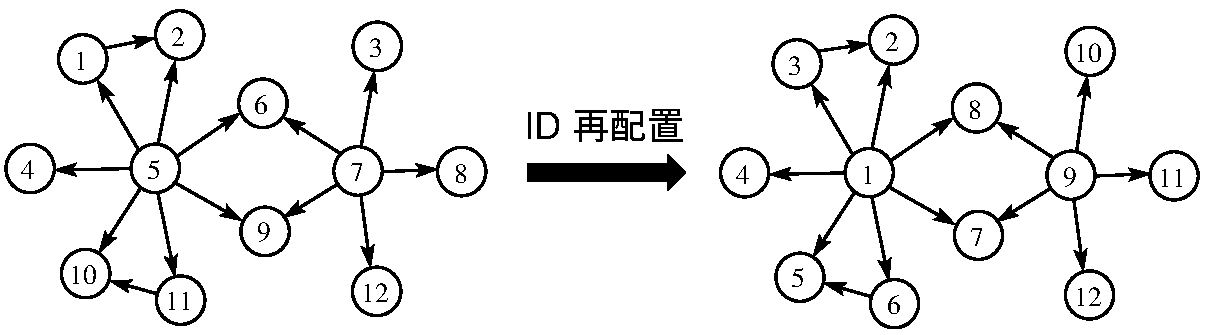
\includegraphics[width=\linewidth]{./figure/reordering_intro.pdf}
  \caption{ノード ID 再配置の例}
  \label{reordering_intro}
\end{figure}
RW で収集したグラフに対しても Reordering は有効であるが,既存の Reordering 手法は対象グラフの
全体構造が把握可能という制約条件が設定されている.
つまり,自律分散グラフ管理環境で既存の Reordering 手法を適用する場合,RW によるグラフ収集が完了するまで Reordering を実行できない.
Reordering を実行するまで収集したグラフはメモリ上で格納し続ける必要があるため,
収集するグラフサイズに比例したメモリ使用が発生してしまう.
\begin{comment}
  並列化による処理時間の減少についての評価も取るのであれば,ここで述べる
\end{comment}
人気コンテンツの周辺グラフなど収集したいグラフサイズが巨大な場合を想定すると,
自律分散グラフ管理環境におけるメモリ使用を抑えた Reorderin 手法が必要となる.

本研究では,自律分散グラフ管理環境においてメモリ使用を抑えるために,RW によるグラフ収集の途中で
部分的に Reordering を実行する手法として Sequential と Dynamic Degree Based Grouping (DDBG) を提案する.
そして,自律分散グラフ管理環境において Sequential, DDBG をそれぞれ実行した時の演算速度向上率,Reordering に伴うメモリ使用量
を明らかにする.
\section{本研究の位置付け}
TO DO

4分割のマトリックス的なやつを示し,SequentialとDBG-EEの立ち位置を,再配置に伴う特徴から明示する.
なぜか画像が表示されないんだがあ

\section{本論文の構成}
第1章では自律分散グラフ管理環境の概要と既存の Graph Reordering 手法の問題点を明示し,自律分散グラフ管理環境を想定した
Graph Reordering 手法の必要性を述べた.第2章では Graph Reordering の技術的な特徴を整理し,Reordering と グラフ演算時のキャッシュミス減少との
関係性について述べる.第3章では本論文の関連研究について述べる.第4章では提案手法である Sequential と DDBG について述べる.第5章では提案手法の
評価を行う.最後に第6章では本論文における結論と今後の課題について述べる.

\chapter{Graph Reordering}
\label{chap:existing_technology}
グラフ演算時にはメモリへの不規則なアクセスによるキャッシュミスが多発する.\cite{wei2016speedup} では,sd1-arc データセット (9,500万ノード,19 億エッジ)
を使用し,代表的なグラフアルゴリズムである 
Breadth-First Search (BFS) \cite{cormen2009introduction},Depth-First Search (DFS) \cite{cormen2009introduction},
Strongly Connected Component (SCC) \cite{sharir1981strong},Shortest Path (SP) \cite{cormen2009introduction},
PageRank (PR),Dominating Set (DS) \cite{cockayne1978domination},Graph Decomposition (Kcore) \cite{batagelj2003m},Graph Diameter (Diam) を
実行したところ, 演算時間全体の内,キャッシュミスに伴うメインメモリへのアクセス時間が占める平均割合は約 70 \% であると報告されている.
図 \ref{cache_miss_ratio}に示されているように,演算時間全体に対し,キャッシュミスに伴うメインメモリへのアクセス時間が占める割合は極めて高い.
つまり,演算時のキャッシュミスを減少させることで,演算時間を減少させることが可能である.
\begin{figure}[t]
  \centering
  %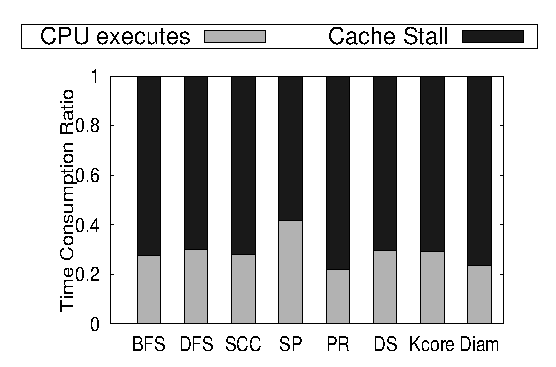
\includegraphics[width=\linewidth]{./figure/cache_miss.pdf}
  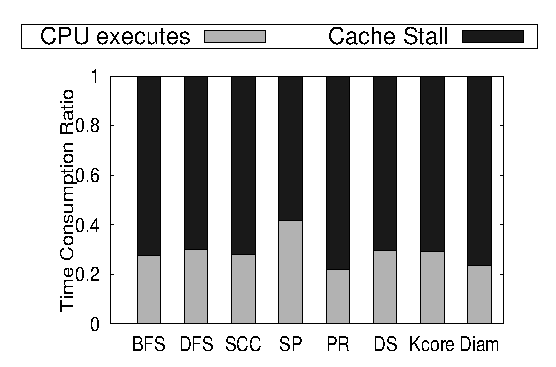
\includegraphics[scale=1.0]{./figure/cache_miss.pdf}
  \caption{演算時間全体に対しキャッシュミスに伴うメインメモリへのアクセス時間が占める割合}
  \label{cache_miss_ratio}
\end{figure}

ノード ID の再配置では,グラフ演算に伴うメモリアクセスの特徴を考慮することで,キャッシュミス減少を実現する.
また,ノード ID の配置を変更するだけなので,グラフアルゴリズムやデータ構造自体を変更する必要はなく,既存のグラフ処理系に対して容易に適用することが可能である.

グラフ演算では各ノードが PR における重要度や BFS における始点からの距離などのアルゴリズム固有の値を保持しており,これらの値はノード ID をインデックスとする配列へ格納される.
%一般に,これらの値は図 \ref{id_index}で示すように,ノード ID をインデックスとする配列に格納される.
図\ref{id_index} にノード ID をインデックスとする配列の例を示す.
\begin{figure}[t]
  \centering
  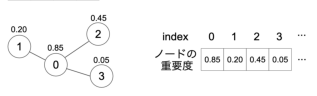
\includegraphics[width=\linewidth]{./figure/id_index.pdf}
  \caption{ノード ID をインデックスとする配列での格納}
  \label{id_index}
\end{figure}
配列はメモリ上で連続した領域を確保するため,ID が連続するノードの値はメモリ上で連続して格納され,ID が近いノードの値は同一キャッシュブロックに属する.
そのため,ノード ID X の値が参照された場合,X 前後の ID を持つノードの値もまとめてキャッシングされる
図\ref{cache_block}にブロック単位でのキャッシングの例を示す.
\begin{figure}[t]
  \centering
  %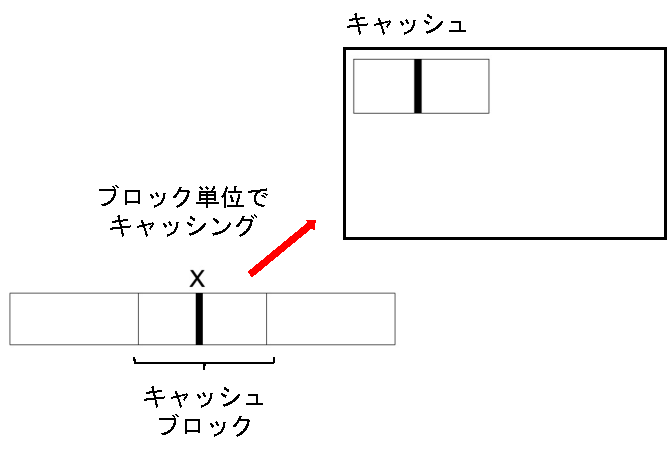
\includegraphics[width=\linewidth]{./figure/cache_block.pdf}
  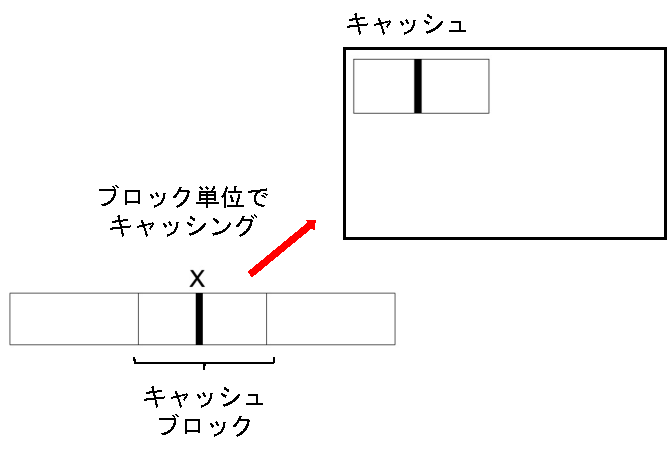
\includegraphics[scale=1.0]{./figure/cache_block.pdf}
  \caption{ブロック単位でのキャッシング}
  \label{cache_block}
\end{figure}
グラフ演算では演算過程において隣接ノードの値を参照とするという操作が繰り返されるため,ノード ID の配置方法によりキャッシュの使用効率も変化する.
そこで,グラフを取得しながらノード ID を再配置するにあたり,特に ID の連続性と演算時のアクセス局所性が重要となる.
\section{ID の連続性}
既存手法では,グラフの全体構造を把握した上で再配置を行うので,全ノードに連続した ID が再配置されることが保証される.
しかし,グラフを取得しながら ID を再配置する場合,再配置する ID が連続的かどうかを考慮する必要がある.
ID が連続するノードの値はメモリ上でも連続して格納されるが,ID の連続性が欠如していると,各ノードの値がメモリ上で点在する形となり,
全ノードを格納するためのキャッシュブロック数が増加してしまう.
キャッシュブロック数の増加に伴い,演算時にアクセス対象となるブロック数も増加し,
キャッシュブロックの書き換えが頻発してしまうためキャッシュミスが増加する.
例えば,図\ref{id_not_consecutive} で示すように,ノード ID が 2, 6, 10, 37, 53 と非連続的で,これら 5 ノードの値を格納するために
必要なブロック数が 3 だとする.
このグラフのノード ID を図\ref{id_consecutive} で示すように再配置する.
ID の連続性を実現した再配置により,同一の 5 ノードを格納するために必要なブロック数が 1 に減少している.
\begin{figure}[t]
  \begin{tabular}{cc}
    \begin{minipage}[t]{0.45\hsize}
      \centering
      %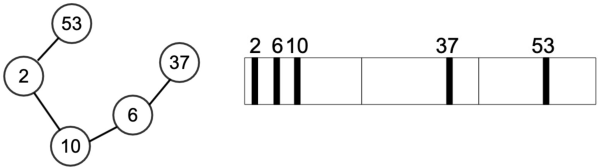
\includegraphics[keepaspectratio, scale=0.50]{./figure/id_not_consecutive.pdf}
      %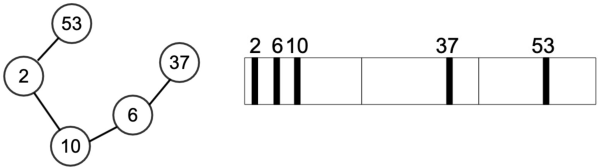
\includegraphics[keepaspectratio, width=7cm]{./figure/id_not_consecutive.pdf}
      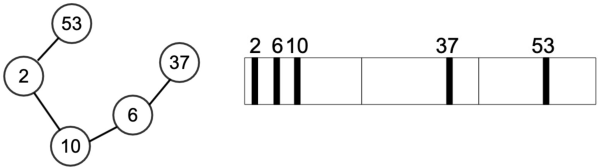
\includegraphics[width=7cm]{./figure/id_not_consecutive.pdf}
      %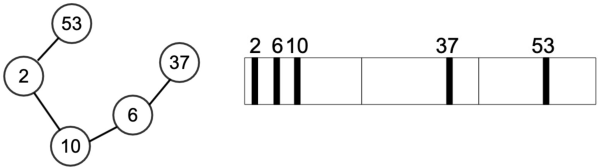
\includegraphics[scale=0.50]{./figure/id_not_consecutive.pdf}
      \caption{ID が非連続的な場合のブロック数}
      \label{id_not_consecutive}
    \end{minipage} &
    \begin{minipage}[t]{0.45\hsize}
      \centering
      %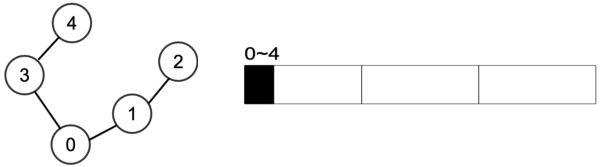
\includegraphics[keepaspectratio, scale=0.50]{./figure/id_consecutive.pdf}
      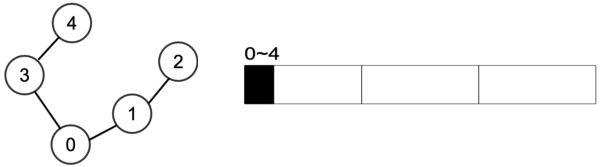
\includegraphics[width=7cm]{./figure/id_consecutive.pdf}
      %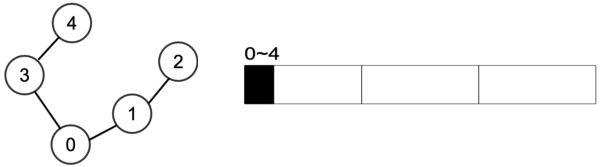
\includegraphics[scale=0.50]{./figure/id_consecutive.pdf}
      \caption{ID が連続的な場合のブロック数}
      \label{id_consecutive}
    \end{minipage}
  \end{tabular}
\end{figure}
\section{演算時のアクセス局所性}
グラフを取得しながら ID を再配置する場合でも,既存手法と同様に演算時のアクセス局所性を考慮する必要がある.
具体的には,演算時に局所的なアクセスが発生するノード群を同一キャッシュブロックに格納しておくことで,
キャッシュの使用効率が向上し,キャッシュミスが減少する.
アクセス局所性は次数による局所性と近接構造による局所性に分類できる.
\subsection{次数による局所性}
実世界グラフは次数分布が冪乗則に従うスケールフリー性と呼ばれる性質を持つ\cite{barabasi1999emergence,faloutsos1999power,clauset2009power}.
スケールフリー性を持つグラフでは,極めて少数のノードが高い次数を持つ一方で,大多数のノードは低い次数を持つ.
グラフ演算における各ノードへのアクセス頻度はそのノードの次数に比例するため,
少数の高次数ノードへアクセスが集中する.
このように,グラフがスケールフリー性を持つ状況では,次数が同程度のノードが同一キャッシュブロックに格納されるように ID を再配置することが有効である.

図\ref{bad_degree_cache} で示すように,同一キャッシュブロック内に次数が大きく異なるノードの値が格納されている場合,
低次数ノードの値は高次数ノードへのアクセスに伴って頻繁にキャッシングされる.
グラフ演算において低次数ノードへのアクセス数は極めて小さいため,
アクセスされにくい値の頻繁なキャッシングはキャッシュの使用効率低下を引き起こす.
一方,図\ref{good_degree_cache} で示すように,同一キャッシュブロック内に同程度の次数を持つノードの値が格納されている場合,
高次数ノードのアクセスに伴い低次数ノードの値がキャッシングされることを防止できる.
これにより,高次数ノードの値を格納しているブロックは演算終了時までキャッシュに格納され続け,
低次数ノードの値を格納しているブロックは必要最低限の回数だけキャッシングされるため,演算時のキャッシュミスが減少する.


\begin{figure}[t]
  \begin{tabular}{cc}
    \begin{minipage}[t]{0.45\hsize}
      \centering
      %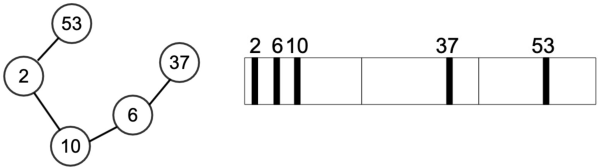
\includegraphics[keepaspectratio, scale=0.50]{./figure/id_not_consecutive.pdf}
      %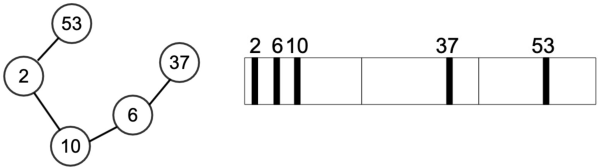
\includegraphics[keepaspectratio, width=7cm]{./figure/id_not_consecutive.pdf}
      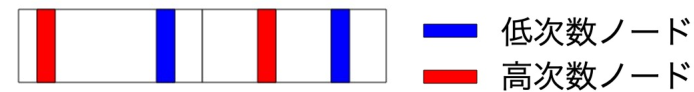
\includegraphics[width=7cm]{./figure/bad_degree_cache.pdf}
      %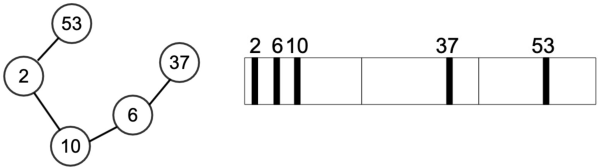
\includegraphics[scale=0.50]{./figure/id_not_consecutive.pdf}
      \caption{ブロック内のノードの次数に差がある場合}
      \label{bad_degree_cache}
    \end{minipage} &
    \begin{minipage}[t]{0.45\hsize}
      \centering
      %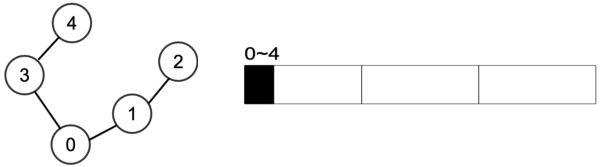
\includegraphics[keepaspectratio, scale=0.50]{./figure/id_consecutive.pdf}
      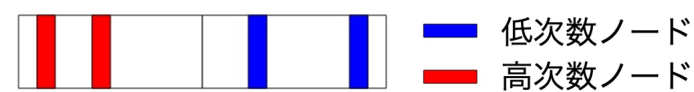
\includegraphics[width=7cm]{./figure/good_degree_cache.pdf}
      %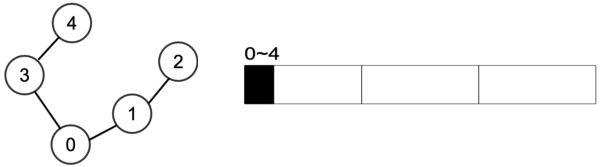
\includegraphics[scale=0.50]{./figure/id_consecutive.pdf}
      \caption{ブロック内のノードの次数が同程度の場合}
      \label{good_degree_cache}
    \end{minipage}
  \end{tabular}
\end{figure}

%なお,次数による局所性に着目した ID 再配置手法として \cite{zhang2017making,faldu2019closer}が提案されている.
\subsection{近接構造による局所性}
実世界グラフはスケールフリー性だけでなく,コミュニティ構造を保有するという特徴を持つ\cite{girvan2002community,leskovec2009community}.
コミュニティとは,グラフ上で密に接続しあっているノードの集合であり,同一コミュニティに所属するノードはグラフ上で極めて近接している.
%コミュニティ内のノード群は密に接続しあっており,グラフ上で極めて近接している.
一般に,グラフ演算では隣接ノードの値を参照するという操作が繰り返されるため,コミュニティ内のノード間で局所的なアクセスが発生する.
そのため,同一コミュニティに属する極めて近接したノード群の値が同一キャッシュブロックに格納されるように ID を再配置することが有効である.

例えば,図\ref{bad_community_cache}で示すように,ID V のノードに対し,その隣接ノードの ID が 2, 37, 53 と離れている場合,
ノード V の隣接ノードの値を参照するためには,3つのキャッシュブロックにアクセスする必要があるとする.
この場合,図\ref{good_community_cache}で示すように,隣接ノードが近い ID を持つように ID を再配置することで,
全隣接ノードが同一キャッシュブロックに格納され,演算時には1つのキャッシュブロックへアクセスするだけでノード V の全隣接ノードの値を参照することが可能となる.
このように,グラフ上で近接しているノードが同一キャッシュブロックへ格納されるように ID を再配置することで,演算全体を通してアクセスする
ブロック数が減少し,キャッシュミスが減少する.
\begin{figure}[t]
  \begin{tabular}{cc}
    \begin{minipage}[t]{0.45\hsize}
      \centering
      %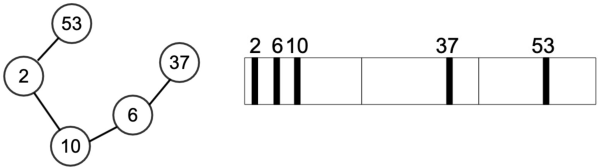
\includegraphics[keepaspectratio, scale=0.50]{./figure/id_not_consecutive.pdf}
      %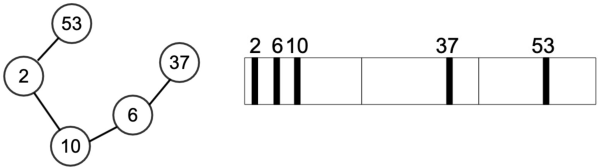
\includegraphics[keepaspectratio, width=7cm]{./figure/id_not_consecutive.pdf}
      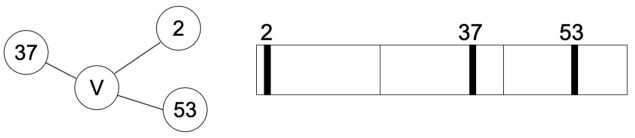
\includegraphics[width=7cm]{./figure/bad_community_cache.pdf}
      %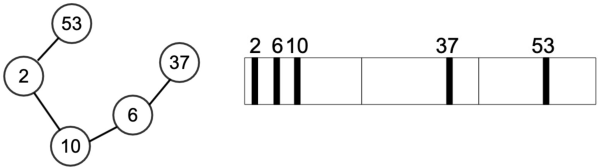
\includegraphics[scale=0.50]{./figure/id_not_consecutive.pdf}
      \caption{近接ノードの ID が離れている場合}
      \label{bad_community_cache}
    \end{minipage} &
    \begin{minipage}[t]{0.45\hsize}
      \centering
      %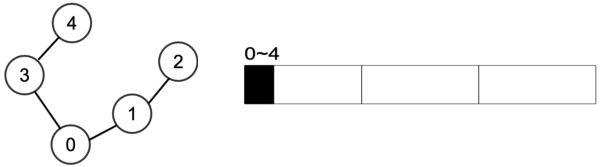
\includegraphics[keepaspectratio, scale=0.50]{./figure/id_consecutive.pdf}
      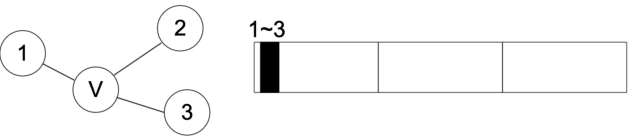
\includegraphics[width=7cm]{./figure/good_community_cache.pdf}
      %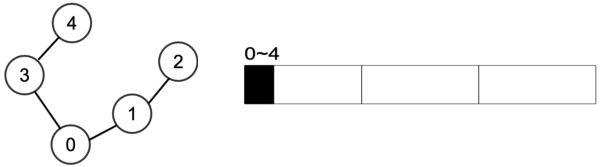
\includegraphics[scale=0.50]{./figure/id_consecutive.pdf}
      \caption{近接ノードの ID が近い場合}
      \label{good_community_cache}
    \end{minipage}
  \end{tabular}
\end{figure}

\section{自律分散グラフ管理環境での課題}
既存手法はグラフの全体構造を把握している前提で議論がされているため,再配置の対象となるノード数は既知である.
予めノード数が判明していることで ID の連続性が保証されているが,グラフ取得が完了するまで全グラフが手元にない状況では
既存手法と同様に ID の連続性を保証することは不可能である.
グラフ取得をしながら ID の連続性を保った再配置を実行するには,取得途中のグラフに対して連続的な ID を再配置し続ける必要がある.
しかし,取得途中のグラフ構造には次数による局所性や近接構造による局所性などの特徴が十分に反映されない可能性が高い.
例えば,取得初期の段階で高次数ノードと判定されたノードが取得完了時点では低次数ノードであると判明する可能性がある点や,
取得途中ではグラフ上の近接構造を正確に把握することが困難な点などが挙げられる.
ID の連続性のみを意識して再配置を行うと演算時のアクセス局所性が損なわれてしまうが,
アクセス局所性のみを意識するとグラフの取得完了を待つコストが増加してしまう.
このように,グラフ取得が完了するまで全グラフが手元にない状況では連続性とアクセス局所性の完全な両立は困難である.

\chapter{関連研究}
\label{chap:related_research}
\section{Gorder}
Gorder\cite{wei2016speedup} は演算時のアクセス局所性に着目し,有向グラフ上で任意の2ノード u, v 間に \textit{neighbor relationship} と \textit{sibling relationship} を定義する.
そして,これらの関係に基づいてノード u, ノード v の近接度合いをスコア化する.
neighbor relationship に基づくスコアでは,ノード u,ノード v が双方向にエッジを張っている場合+2,
ノード u,ノード v の一方から他方へエッジが張られている場合+1,ノード u,ノード v 間にエッジが張られていない場合+0 となる.
また,sibling relationship に基づくスコアでは,ノード u,ノード v が共通のノード x からエッジを張られている場合+1 となり,
ノード x の数に応じてスコアが加算されていく.
neighbor relationship を図\ref{neighbor} に,sibling relationship を図\ref{sibling} に示す. 
\begin{figure}[t]
  \begin{tabular}{cc}
    \begin{minipage}[t]{0.45\hsize}
      \centering
      %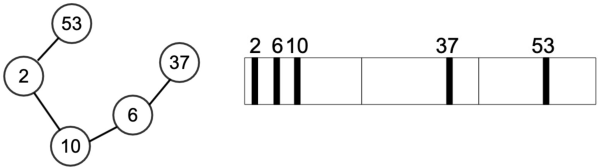
\includegraphics[keepaspectratio, scale=0.50]{./figure/id_not_consecutive.pdf}
      %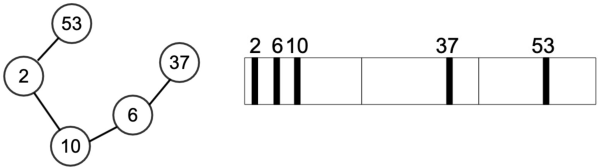
\includegraphics[keepaspectratio, width=7cm]{./figure/id_not_consecutive.pdf}
      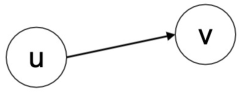
\includegraphics[width=6.5cm]{./figure/neighbor.pdf}
      %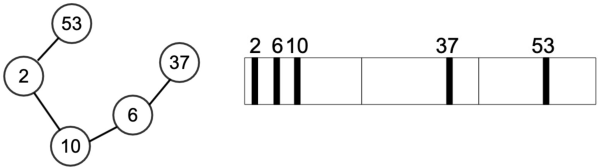
\includegraphics[scale=0.50]{./figure/id_not_consecutive.pdf}
      \caption{neighbor relationship}
      \label{neighbor}
    \end{minipage} &
    \begin{minipage}[t]{0.45\hsize}
      \centering
      %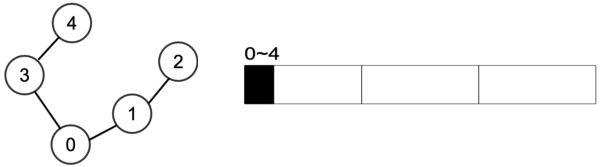
\includegraphics[keepaspectratio, scale=0.50]{./figure/id_consecutive.pdf}
      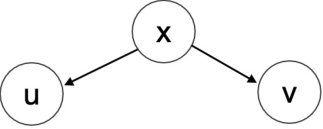
\includegraphics[width=7cm]{./figure/sibling.pdf}
      %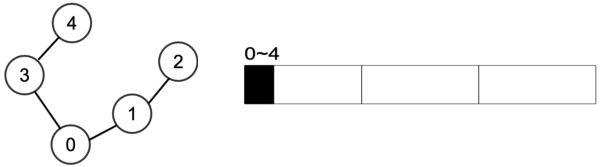
\includegraphics[scale=0.50]{./figure/id_consecutive.pdf}
      \caption{sibling relationship}
      \label{sibling}
    \end{minipage}
  \end{tabular}
\end{figure}
ここで,neighbor relationship に基づくスコアを $S_{n}(u,v)$,sibling relationship に基づくスコアを $S_{s}(u,v)$としたとき,
ノード u,ノード v のスコア $S(u,v)$ は(\ref{gorder_score})式で定義される.
\begin{equation}
  S(u,v) = S_{n}(u,v) + S_{s}(u,v) \label{gorder_score}
\end{equation}
そして,ノード u,ノード v の ID がそれぞれ $\phi(u)$,$\phi(v)$に変換される時,
(\ref{gorder})式で定義する $F(\phi)$ を最大化する ID 配置 $\phi$ に基づいて再配置を実行する.
\begin{equation}
  F(\phi) = \sum_{0<\phi(v)-\phi(u)\leq3}^{} S(u,v) \label{gorder}
\end{equation}
なお,図\ref{reordering_intro} は Gorder の例を示しており,(\ref{gorder})式で定義される$F(\phi)$ を最大化するように ID が再配置されている.
Gorder はグラフ演算速度の向上率という観点では最良の ID 再配置手法だが,前処理の時間コストが大きすぎるため非実用的と指摘されている\cite{balaji2018graph, faldu2019closer}.
\section{Degree Sorting}
DegreeSorting は次数による局所性のみに着目し,高次数ノードから昇順の ID を再配置していく.
図\ref{Original} で示す 12 ノードを Degree Sorting で再配置する場合の例を図\ref{degree_sorting} で示す.
なお,図\ref{Original} では,平均次数 20 を越えるノードは薄い赤色,平均次数の 2 倍である 次数 40 を越えるノードは濃い赤色で示されている.
次数に基づくソードにより,ID が近いノードは同程度の次数であることが保証されるため,次数による局所性を十分に考慮することができる.
しかし,\cite{balaji2018graph, faldu2019closer} などで元の ID が近いノードはグラフ上で近接していることが明らかになっている.
そのため,次数によるソートでグラフの近接構造を表す情報が失われてしまい,近接構造による局所性を考慮することが不可能となる.
\begin{figure}[t]
  \centering
  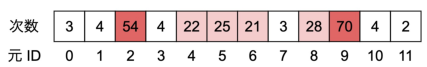
\includegraphics[width=\linewidth]{./figure/original.pdf}
  \caption{再配置対象のノード ID と次数情報}
  \label{Original}
\end{figure}
\begin{figure}[t]
  \centering
  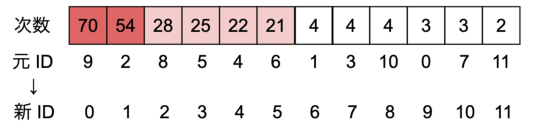
\includegraphics[width=\linewidth]{./figure/degree_sorting.pdf}
  \caption{Degree Sorting による再配置の例}
  \label{degree_sorting}
\end{figure}
\section{Hub Sorting}
Hub Sorting \cite{zhang2017making} は,Degree Sorting と同様に次数による局所性に着目しているが,高次数ノードのみ次数に基づくソートを実行し ID を再配置している.
これにより,低次数ノードでは近接構造による局所性を維持しつつ,アクセスが集中する高次数ノードでは次数による局所性を考慮している.
Hub Sorting では,平均次数以上の次数を持つノードを高次数ノードとみなしているが,
実世界グラフおいて平均次数以上のノードに接続しているエッジは全体の 80 - 90 \% を占める\cite{faldu2019closer}.
そのため,高次数ノードにおいても近接構造による局所性を考慮した ID 再配置を実行する必要があるが,
Hub Sorting による再配置では高次数ノードでの近接構造による局所性を考慮できていないという問題点が存在する.
図\ref{hubclustering} で Hub Sorting による再配置の例を示すが,平均次数 20 を越える高次数ノード内で元の ID の順序が保たれていないことが確認できる.
\begin{figure}[t]
  \centering
  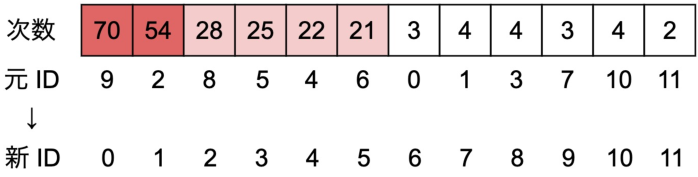
\includegraphics[width=\linewidth]{./figure/hubsorting.pdf}
  \caption{Hub Sorting による再配置の例}
  \label{hubsorting}
\end{figure}
\section{Hub Clustering}
Hub Clustering \cite{balaji2018graph} は,Hub Sorting における問題点に着目し,高次数ノード内でソートを行わずに元の ID 順を保った再配置を行うことで
高次数ノードでの近接構造による局所性を考慮している.
しかし,実世界グラフはスケールフリー性を持つため,平均次数以上のノード内でも次数分布には大きな偏りが発生する.
そのため,Hub Clustering では,高次数ノード内での次数分布の偏りを考慮した ID 再配置が行えていないという問題点が存在する.
図\ref{hubclustering} で Hub Clustering による再配置の例を示す.
Hub Sorting と比較して高次数ノード内でも元の ID 順が保たれているが,次数 54 と次数 70 のノードに連続した ID を再配置できていないことが確認できる.
\begin{figure}[t]
  \centering
  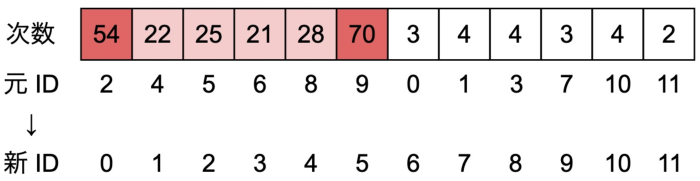
\includegraphics[width=\linewidth]{./figure/hubclustering.pdf}
  \caption{Hub Clustering による再配置の例}
  \label{hubclustering}
\end{figure}
\section{Degree Based Grouping (DBG)}
\label{dbg}
Hub Sorting や Hub Clustering で問題が生じる主要な要因は,平均次数というただ1つの境界値に基づき高次数ノードと低次数ノードを二分しているからである.
そこで,DBG \cite{faldu2019closer}はグラフの平均次数$\mathbb{A}$に基づき,[0,$\mathbb{A}$/2),[$\mathbb{A}$/2,$\mathbb{A}$),[$\mathbb{A}$,2$\mathbb{A}$),[2$\mathbb{A}$,4$\mathbb{A}$),
[4$\mathbb{A}$,8$\mathbb{A}$),[8$\mathbb{A}$,16$\mathbb{A}$),[16$\mathbb{A}$,32$\mathbb{A}$),[32$\mathbb{A}$,$\infty$)
と 次数の範囲が異なる 8 グループを定義し,各ノードを次数でグループ分けする.
HubSorting や HubClustering は,[0,$\mathbb{A}$),[$\mathbb{A}$,$\infty$) の 2 グループしか定義されていないため,
高次数ノード内での次数分布の偏りに対応できていないが,DBG では 8 グループ定義することで次数分布の偏りに対応している.
そして,高次数のグループから元の ID 順を保って昇順の連続した ID を再配置することで次数による局所性と近接構造による局所性の双方を考慮している.
DBG による再配置の例を図\ref{dbg} で示す.
\begin{figure}[t]
  \centering
  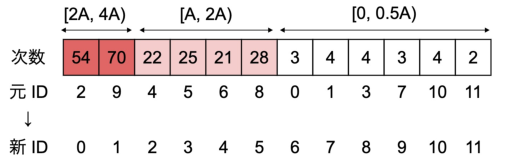
\includegraphics[width=\linewidth]{./figure/dbg.pdf}
  \caption{DBG による再配置の例}
  \label{sec:dbg}
\end{figure}
\section{まとめ}
本章では,既存の代表的な ID 再配置手法として,Gorder,Degree Sorting,Hub Sorting,Hub Clustering を紹介した.
また,本章で紹介した手法以外にも,Rabbit Order \cite{arai2016rabbit},ReCall \cite{lakhotia2017recall},Slash Burn \cite{kang2011beyond},
METIS \cite{karypis1998multilevelk} などの手法が提案されている.
しかし,既存手法はグラフの全体構造が把握可能という前提のもと議論されている.
そのため,グラフ取得の完了まで全グラフが手元にない状況へ既存手法を適用することは困難であり,グラフを取得しながら ID を再配置するという手法は存在しない.

\chapter{自律分散グラフ管理環境における Reordering}
\label{chap:design}
%本章では,提案手法である ID の連続性を意識した Sequential と
%演算時のアクセス局所性を意識した DBG Early Estimation (DBG-EE) についてそれぞれ説明する.
本研究では,グラフを取得しながらノード ID を再配置する手法として,Sequential と DBG Early Estimation (DBG-EE) を提案する.
図\ref{research_position} で示すように,Sequential は ID の連続性を意識し,DBG-EE は演算時のアクセス局所性を意識している.
Sequential では ID の連続性を保証するために RW で出会ったノード順に昇順の連続した ID を再配置する.
DBG-EE では 図\ref{degree_appro} で示すように,RW 途中での取得グラフにおける次数分布が RW 終了時点の取得グラフにおける次数分布に近似する性質に着目し ID を再配置する.
具体的には,既存手法でノードの次数情報しか必要とせず,前処理コストと演算速度向上のバランスに優れる DBG \cite{faldu2019closer} をもとに再配置を行う.
\begin{figure}[t]
  \centering
  %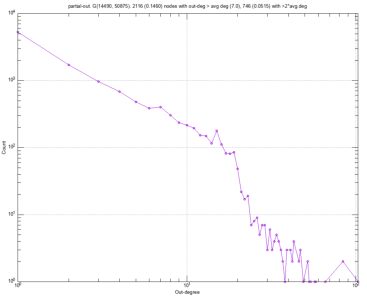
\includegraphics[width=\linewidth]{./figure/degree_appro.pdf}
  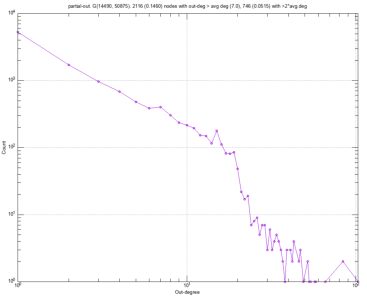
\includegraphics[width=12cm]{./figure/degree_appro.pdf}
  \caption{取得途中のグラフと取得完了時のグラフにおける次数分布}
  \label{degree_appro}
\end{figure}
\section{Sequential}
Sequential では,RW によるグラフ取得において新しく出会ったノード順に連続した昇順の ID を再配置する.
再配置に伴い新たな ID が割り振られる度に,元の ID と新たな ID の対応関係をマッピングテーブルへ登録する.
このマッピングテーブルを参照することで,RW 途中での訪問先ノードがすでに再配置済みか即座に判定することが可能となっている.

\subsection{RW の訪問順に基づく ID 再配置}
Sequential による ID 再配置の具体例を 図\ref{sequential-rw} で示すように 1 → 4 の順でノードを移動しグラフを取得する場合で考える.
このとき,図\ref{sequential} に示す手順で ID の再配置と再配置済みグラフの更新が行われる.
まず,RW 開始時点で再配置されたノードは存在しないため,1回目の移動に伴い ID 10 の始点ノードと ID 6 のノードに
それぞれ ID 0 と ID 1 が再配置される.
そして,ID 10 → ID 0,ID 6 → ID 1 という対応関係をマッピングテーブルに登録し,ID 0 のノードと ID 1 のノード間にエッジが張られていることを再配置済みのグラフ構造として保持する.
次に,2回目の移動に伴い ID 37 というノードへ辿り着くが,マッピングテーブルに ID 37 の対応関係は登録されていない.
そこで,新たに ID 37 のノードへ ID 2 を再配置し,ID 37 → ID 2 という対応関係をマッピングテーブルへ登録する.
そして,マッピングテーブルの参照により ID 6 → ID 1,ID 37 → ID 2 という対応関係が分かるので,ID 1 のノードと ID 2 のノード間にエッジが張られていることを再配置済みのグラフへ反映させる.
以降も同様にマッピングテーブルの参照・登録及び再配置済みグラフの更新を RW 終了まで繰り返す.
\begin{figure}[t]
  \centering
  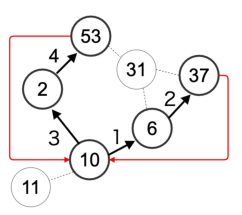
\includegraphics[width=7cm]{./figure/sequential-rw.pdf}
  \caption{1→4 の順にノードを移動しグラフを取得}
  \label{sequential-rw}
\end{figure}
\begin{figure}[t]
  \centering
  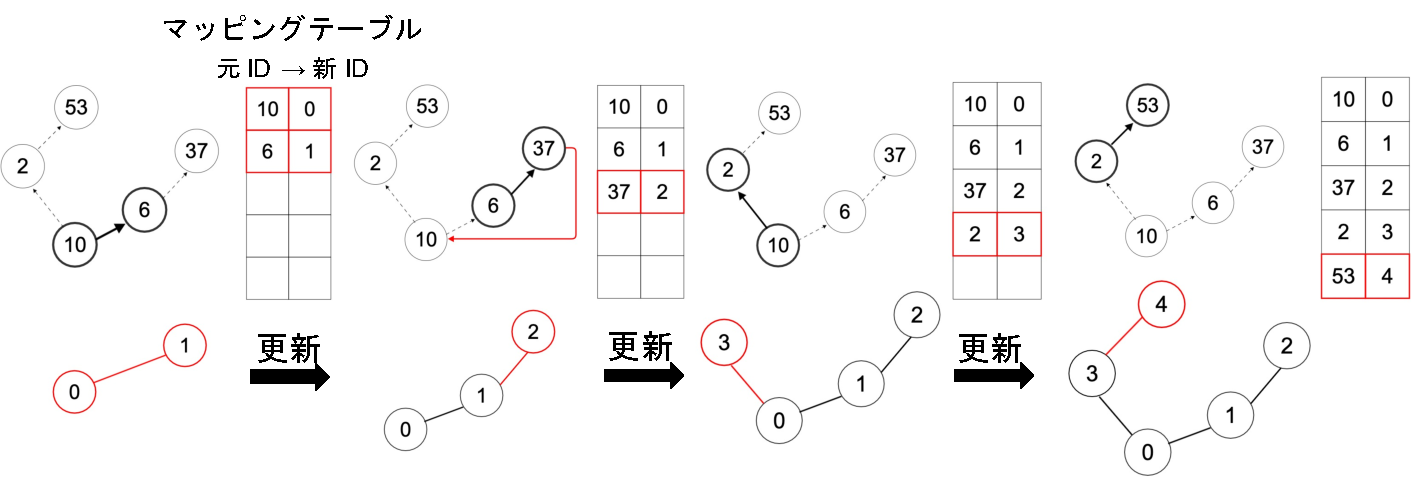
\includegraphics[width=\linewidth]{./figure/sequential.pdf}
  \caption{Sequential におけるノード ID 再配置}
  \label{sequential}
\end{figure}

\subsection{メモリ使用量を抑えたグラフ構造の保持}
Sequential では RW でノードを移動する度にマッピングテーブルの参照・登録及び再配置済みグラフの更新を行うことで
再配置待ちのグラフ構造を保持する必要を無くし,メモリ使用量を削減している.
図\ref{sequential_bad_memory}で示すように,グラフを取得してから再配置を行う場合は取得完了時のグラフと再配置済みのグラフを
メモリ上で保持する必要がある.
しかし,Sequential による再配置では図\ref{sequential_good_memory}で示すように,RW で移動した1エッジと再配置済みのグラフを保持するだけで良く,
1エッジを保持するためのメモリ使用量は取得完了時のグラフを保持するためのメモリ使用量より遥かに小さい.
\begin{figure}[t]
  \begin{tabular}{cc}
    \begin{minipage}[t]{0.45\hsize}
      \centering
      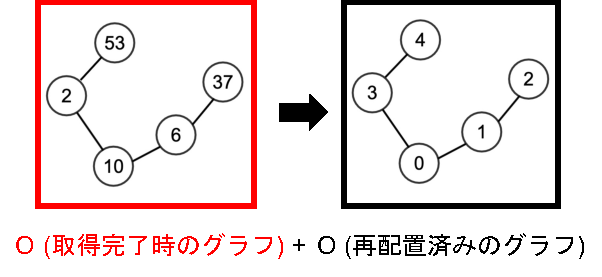
\includegraphics[width=7cm]{./figure/sequential_bad_memory.pdf}
      \caption{取得が完了してから再配置する場合の\\メモリ使用量}
      \label{sequential_bad_memory}
    \end{minipage} &
    \begin{minipage}[t]{0.45\hsize}
      \centering
      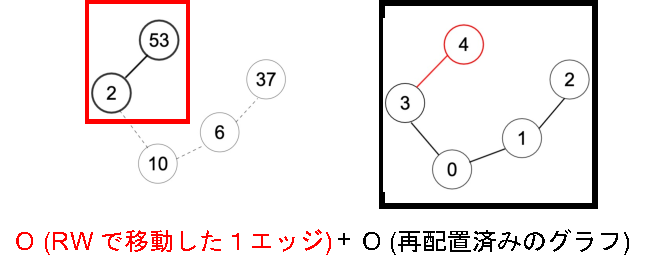
\includegraphics[width=7cm]{./figure/sequential_good_memory.pdf}
      \caption{Sequential において再配置に必要な\\メモリ使用量}
      \label{sequential_good_memory}
    \end{minipage}
  \end{tabular}
\end{figure}
\subsection{近接構造による局所性の部分的な実現}
Sequential は RW によるグラフ取得の途中で出会ったノード順に連続した ID を再配置するため ID の連続性は保証される.
さらに,RW では始点に戻る場合を除き,隣接ノードにしか移動しないため,図\ref{sequential-rw}で示す 1 → 2 のような移動の場合,
隣接ノードへ連続した ID が再配置される.
このように,Sequential では RW による移動の仕方によって隣接ノードへ連続した ID の再配置が可能となり,
近接構造によるアクセス局所性を考慮した再配置が部分的に実現されている.

\section{DBG Early Estimation (DBG-EE)}
DBG-EE では,RW によるグラフ取得の途中でノードを次数に基づきグループ分けし,各グループ毎に ID を再配置する.
なお,DBG-EE では DBG におけるグループ定義を踏襲し,グラフの平均次数$\mathbb{A}$に基づき,[0,$\mathbb{A}$/2),[$\mathbb{A}$/2,$\mathbb{A}$),[$\mathbb{A}$,2$\mathbb{A}$),[2$\mathbb{A}$,4$\mathbb{A}$),
[4$\mathbb{A}$,8$\mathbb{A}$),[8$\mathbb{A}$,16$\mathbb{A}$),[16$\mathbb{A}$,32$\mathbb{A}$),[32$\mathbb{A}$,$\infty$)
と 8 グループを定義する.
%ここで,高次数ノードが属する[32$\mathbb{A}$,$\infty$)側から順にグループ0,グループ1..,と名称を付けておく.
取得途中でノードをグループ分けし ID を再配置するには,予め各グループが再配置に使用する ID の範囲を定めておく必要がある.
そこで,DBG-EE では取得初期の段階で各グループのグループサイズを推定し,推定したサイズに基づいて各グループが再配置に使用する ID の範囲を決定する.
また,DBG-EE では取得途中で再配置を実行し,再配置済みのグラフへ反映が完了した時点で取得したグラフを破棄する.
これにより,取得完了まで再配置待ちのグラフを保持し続ける必要が無くなり,メモリ使用量が削減される.
さらに,グラフ取得と ID の再配置を並列して行うことで,グラフ取得を待つだけの時間が減少し,時間コストが削減される.
\subsection{グループサイズの早期推定}
全体で N 回 RW を実行する中で M 回毎に再配置を実行する場合,再配置は N/M 回実行される.
そこで,DBG-EE では1回目の再配置実行時のグループ分け結果に基づき各グループサイズを N/M 倍し,その値を各グループの推定サイズとみなす.
なお,グループ分けを実行する際には取得途中のグラフにおける平均次数を使用する.
図\ref{estimation_size} で示すように,1回目のグループ分けにより x 個のノードがグループ0へ割り振られた場合,グループ0の推定サイズは x $\times$ N/M となる.

\begin{figure}[t]
  \centering
  %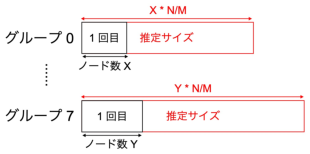
\includegraphics[width=\linewidth]{./figure/estimated_group_size.pdf}
  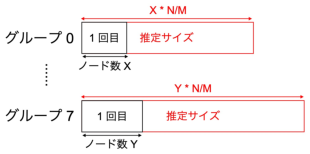
\includegraphics[width=10cm]{./figure/estimated_group_size.pdf}
  \caption{グループサイズの早期推定}
  \label{estimation_size}
\end{figure}
\subsection{推定サイズに基づく ID の範囲決定}
\begin{figure}[t]
  \centering
  %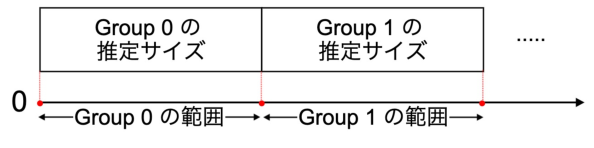
\includegraphics[width=\linewidth]{./figure/group_id_range.pdf}
  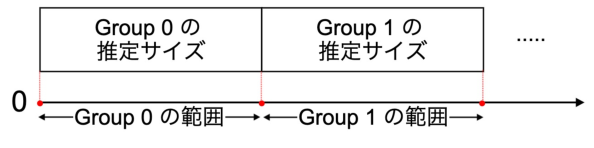
\includegraphics[width=10cm]{./figure/group_id_range.pdf}
  \caption{推定サイズに基づく ID の範囲決定}
  \label{degree_appro}
\end{figure}
\subsection{部分的な取得グラフの破棄}
\begin{figure}[t]
  \centering
  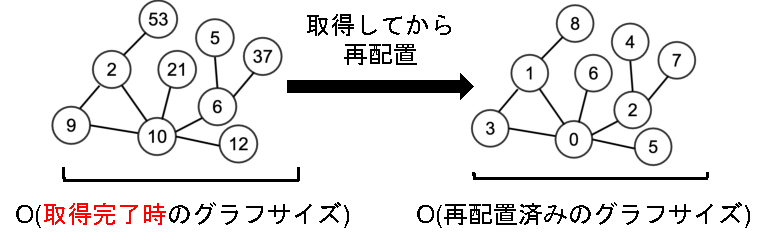
\includegraphics[width=\linewidth]{./figure/dbg-ee_bad_memory.pdf}
  \caption{取得途中のグラフと取得完了時のグラフにおける次数分布}
  \label{degree_appro}
\end{figure}
\begin{figure}[t]
  \centering
  \includegraphics[width=\linewidth]{./figure/dbg-ee_good_memory.pdf}
  \caption{取得途中のグラフと取得完了時のグラフにおける次数分布}
  \label{degree_appro}
\end{figure}
\subsection{グラフ取得と再配置の並列処理}
\begin{figure}[t]
  \centering
  \includegraphics[width=\linewidth]{./figure/dbg-ee_para.pdf}
  \caption{取得途中のグラフと取得完了時のグラフにおける次数分布}
  \label{degree_appro}
\end{figure}

\begin{comment}
\chapter{プロトコル詳細}
\label{chap:protocol}
\input{05-protocol}
\end{comment}

\begin{comment}
\chapter{実装}
\label{chap:implementation}
\section{概要}
言語は C++17 を用いた.ここでは主に以下の 3 点について述べる.
\begin{itemize}
  \item グラフ取得の基本的な実装
  \item Sequential における再配置の実装
  \item DBG-EE における再配置の実装 
\end{itemize}
\section{グラフ取得の基本的な実装}
\subsection{グラフ構造を保持するためのデータ構造}
\label{graph_data}
まず,取得したグラフを保持するためのデータ構造について述べる.
本手法では隣接リストによるグラフ表現として,始点ノードの ID をキー,終点ノードの集合をペアとするハッシュ連想配列を採用している.
%実際に使用したデータ構造をソースコード \ref{data_structure} に示す.
\begin{lstlisting}[caption=グラフ構造, label=data_structure]
  typedef unordered_map<unsigned int, vector<unsigned int>> Graph; 
\end{lstlisting}

\subsection{RW によるグラフ取得}
RW 中は滞在ノードにおいて 0 以上 1 以下の乱数値を発生させ,乱数値が確率 α を下回った場合は始点へ移動する.
また,α を下回らない場合でも,滞在ノードの出次数が 0 の場合は始点へ移動する.
乱数値が α を下回らず,滞在ノードの出自数が 1 以上の場合は,
滞在ノードの隣接ノード群からランダムに 1 ノードを選択し,そのノードへ移動する.
このような移動を繰り返す中で,滞在ノードと移動先ノードの間にエッジが存在するかを毎回確認する.
そして,エッジが存在していない場合は取得グラフに新たなエッジとして追加する.
\begin{lstlisting}[caption=RW によるグラフ取得, label=rw_graph_get]
  // All_Graph : データセットを保持するグラフ
  // Get_Graph : RW により取得したグラフ
  Graph Get_Graph, All_Graph;

  // 0 以上 1 以下の乱数生成 
  random_device seed_gen;
  mt19937 engine(seed_gen());
  uniform_real_distribution<> dist(0,1.0);
  // src : 始点ノード,dst : 終点ノード
  unsigned int RW_num, RW_count, src, dst;
  // RW の始点
  unsigned int start_node;
  // RW で始点に戻る確率
  float return_prob;

  while (RW_count < RW_num) {
    if (dist(engine) < return_prob) {
      src = start_node;
      RW_count++;
      continue;
    } else {
      // src から進めない場合,始点へ戻る
      if (All_Graph[src].size() == 0) {
        src = start_node;
        RW_count++;
        continue;
      } else {
        // 移動先として隣接ノード群からランダムに1ノード選択
        dst = (All_Graph[src]).at(engine() % All_Graph[src].size());
        // src -> dst にエッジが存在しない場合,Get_Graph へ登録
        if (find(Get_Graph[src].begin(), Get_Graph[src].end(), dst) == Get_Graph[dst].end()) {
        }
        src = dst;
      }
    }
  }
\end{lstlisting}
\section{Sequential における再配置の実装}
Sequential では RW の途中で出会ったノード順に昇順の連続した ID を再配置する.
再配置が行われた場合,マッピングテーブルに ID の対応関係が登録される.
ここで,マッピングテーブルの実装として,元の ID をキー,新たな ID をペアとするハッシュ連想配列を採用している.
\begin{lstlisting}[caption=マッピングテーブル, label=mapping_table]
  typedef unordered_map<unsigned int, unsigned int> Mapping;
\end{lstlisting}

実際の処理では,RW で 1 エッジ移動する度にマッピングテーブルの参照・登録を行うことで,ID が再配置された形でグラフ構造を保持する.
コード \ref{sequential_code} に Sequential における再配置の実装を示す.
この処理はコード \ref{rw_graph_get} における 30 - 32行目に代わって実行される. 
\begin{lstlisting}[caption=Sequential における再配置, label=sequential_code]
  // Sequential_Mapping : Sequential におけるマッピングテーブル
  // 次の移動先ノードが再配置済みか確認 
  if (Sequential_Mapping.count(dst) == 0) {
    Sequential_Mapping[dst] = Sequential_Mapping.size();
  }
  // 再配置された ID でグラフ構造を保持
  mapped_src = Sequential_Mapping[src];
  mapped_dst = Sequential_Mapping[dst];
  if (find(Mapped_Graph[mapped_src].begin(), Mapped_Graph[mapped_src].end(), mapped_dst) == Mapped_Graph[mapped_src].end()) {
    Mapped_Graph[mapped_src].push_back(mapped_dst);
  }
\end{lstlisting}
\section{DBG-EE における再配置の実装}
DBG-EE でも Sequential と同様にコード \ref{mapping_table} で示したマッピングテーブルを使用する.
また,グループサイズの早期推定によって各グループが使用する ID の範囲を決定するが,
再配置が進み,使用できる ID の範囲が狭まった場合でも各グループが使用できる範囲を把握しておく必要がある.
そこで,各グループが使用できる ID の最小値と最大値を保存しておくために,最小値と最大値の組を要素とする動的配列を使用する.
\begin{lstlisting}[caption=グラフ構造, label=data_structure]
  typedef vector<pair<unsigned int, unsigned int>> Group; 
\end{lstlisting}

新たな ID を再配置する場合は,次数に応じて分類されたグループで使用可能な最小の ID を使用する.
そして,最小値をインクリメントすることで次に使用する ID を設定する.
再配置後は ID の対応関係をマッピングテーブルへ登録する.

\begin{lstlisting}[caption=DBG-EE における再配置, label=dbgee-reordering]
// 新たな ID を再配置する関数
void Mapping_id(Mapping & DBGEE_Mapping, Group & DBGEE_Group, unsigne
d int original_id, int deg, float ave_deg)
{
  if (deg > 32 * ave_deg) {
    DBGEE_Mapping[original_id] = DBGEE_Group.at(0).first++;
  } else if (deg > 16 * ave_deg && deg < 32 * ave_deg) {
    DBGEE_Mapping[original_id] = DBGEE_Group.at(1).first++;
  } else if (deg > 8 * ave_deg && deg < 16 * ave_deg) {
    DBGEE_Mapping[original_id] = DBGEE_Group.at(2).first++;
  } else if (deg > 4 * ave_deg && deg < 8 * ave_deg) {
    DBGEE_Mapping[original_id] = DBGEE_Group.at(3).first++;
  } else if (deg > 2 * ave_deg && deg < 4 * ave_deg) {
    DBGEE_Mapping[original_id] = DBGEE_Group.at(4).first++;
  } else if (deg > 1 * ave_deg && deg < 2 * ave_deg) {
    DBGEE_Mapping[original_id] = DBGEE_Group.at(5).first++;
  } else if (deg > 0.5 * ave_deg && deg < 1 * ave_deg) {
    DBGEE_Mapping[original_id] = DBGEE_Group.at(6).first++;
  } else {
    DBGEE_Mapping[original_id] = DBGEE_Group.at(7).first++;
  }
}
\end{lstlisting}

RW 一定回数毎に再配置を行う時,まず取得グラフの平均次数を求める.
ここで,全エッジ数を全始点数で割った出次数の平均を平均次数として採用している.
次に,取得グラフに含まれる全ノードを ID に基づいてソートし,再配置が済んでいないノードはコード \ref{dbgee-reordering} により再配置を実行する.
そして,再配置が済んだ形でグラフ構造の更新を行う.
最後に,処理が終了した段階で取得グラフを破棄することで空間コストを削減している.
\begin{lstlisting}
// 再配置した形でグラフ構造を更新する関数
void DBGEE(Graph & Partial_Graph, Graph & Mapped_Graph, Group & DBGEE_Group, Mapping & DBGEE_Mapping)
{
  unsigned int edge_num = 0;
  for (auto & [src, dsts] : Partial_Graph){
    edge_num += dsts.size();
  }
  // 平均次数を求める
  float ave_deg = static_cast<float>(edge_num)/Partial_Graph.size();

  // 全ノードを ID に基づいてソート
  vector<unsigned int> v_sorted;
  for (auto & [src, dsts] : Partial_Graph){
    v_sorted.push_back(src);
    for (auto dst : dsts) {
      v_sorted.push_back(dst)
    }
  }
  sort(v_sorted.begin(), v_sorted.end());

  // 再配置が済んでいないノードを再配置
  for (auto & node : v_sorted) {
    if (DBGEE_Mapping.count(node) == 0) {
      Mapping_id(DBGEE_Mapping, DBGEE_Group, node, Partial_Graph[node].size(), ave_deg);
  }

  unsigned int mapped_src, mapped_dst;
  for (auto [src, dsts] : Partial_Graph) {
    mapped_src = DBGEE_Mapping[src];
    for (auto & dst : dsts) {
      mapped_dst = DBGEE_Mapping[dst];
      if (find(Mapped_Graph[mapped_src].begin(), Mapped_Graph[mapped_src].end(), mapped_dst) == Mapped_Graph[mapped_src].end()) {
        Mapped_Graph[mapped_src].push_back(mapped_dst);
      }
    }
  }
  // 再配置が完了した時点で取得グラフを破棄
  Partial_Graph.clear();
}
\end{lstlisting}


\end{comment}

\chapter{評価}
\label{chap:evaluation}
\section{実験の目的}
本研究では,RW によるグラフ取得をしながらノード ID を再配置する手法として,Sequential と DBG-EE を提案した.
そこで,実世界グラフのデータセットに対して Sequential 及び DBG-EE を適用した場合の効果を実験から明らかにする.
具体的には,グラフ取得の完了を待たないことによる空間・時間コストの変化及びグラフ演算時間の減少率に着目する.
\section{実験概要}
\subsection{データセット}
実世界グラフのデータセットとして,スタンフォード大学が提供するグラフデータセットライブラリ SNAP \cite{snapnets} 内の 
Pokec Social Network \cite{takac2012data} を使用した.
表 \ref{dataset} に Pokec Social Network のグラフ情報を示す.
90 \% 有効直径とはノード間の最短距離の分布において 90 パーセンタイルに相当する値であり,
任意のノード間で最短距離が 5.2 以下となる確率が 90 \% であることを意味している.
\begin{table}[t]
  \begin{center}
    \caption{Pokec Social Network の概要}
    \begin{tabular}{cc} \toprule
      ノード数 & 1,632,803 \\
      エッジ数 & 30,622,564 \\
      90 \% 有効直径 & 5.2 \\ \bottomrule
    \end{tabular}
    \label{dataset}
  \end{center}
\end{table}

\subsection{パラメータの決定方法}
まず,RW 回数 N の決定方法について述べる.
表 \ref{rw_graph} で示すように,全体グラフのエッジ数に対する取得グラフのエッジ数は N = 100 万 のとき約 5 \%, N = 300 万 のとき約 10 \% となることが
実験的に明らかになった.
5 \% - 10 \% 程度のエッジを取得するという状況は全体グラフの一部を取得するという前提に矛盾しないと
判断し,N = 100 万,300 万をパラメータとして採用した.

次に,始点へ戻る確率 α の決定方法について述べる.
一般に,RW において始点に戻るまでの平均経路長は 1/α であることが知られている.
この平均経路長を 90 \% 有効直径と同程度に設定することで,始点の周辺グラフだけを密に取得し,
全体グラフの構造が失われる状況を回避できる.
表 \ref{dataset} で示すように,Pokec Social Network の 90 \% 有効直径は約 5 なので,α = 0.2 を
採用することで平均経路長と 90 \% 有効直径を同程度に設定した. 

表 \ref{parameter} に全パラメータの値を示す.
M は DBG-EE における再配置実行間隔に対応している.
なお,RW の開始点としてグラフ上の最高次数ノードを採用した.
\begin{table}[t]
  \begin{center}
    \caption{RW 回数と取得したエッジ数の割合の関係}
    \begin{tabular}{cccc} \toprule
      RW 回数 & ノード数 & エッジ数 & 取得したエッジ数の割合 \\ \hline
      100 万回 & 435,934 & 1,411,607 & 4.61 \% \\
      300 万回 & 686,506 & 3,409,700 & 11.3 \% \\ \bottomrule
    \end{tabular}
    \label{rw_graph}
  \end{center}
\end{table}
\begin{table}[t]
  \begin{center}
    \caption{各パラメータの値}
    \begin{tabular}{cc} \toprule
      N & 100 万, 300 万 \\
      M & 1 万,10 万 \\
      α & 0.2 \\ \bottomrule
    \end{tabular}
    \label{parameter}
  \end{center}
\end{table}


\subsection{対象とするグラフ演算}
RW で取得したグラフに対して PageRank (PR) と Personalized PageRank (PPR) を実行した.
なお,PR の計算には Ligra \cite{shun2013ligra} を,PPR の計算には FORA \cite{wang2017fora} を使用した.

\section{評価概要}
評価項目は以下の 3 点である.
\begin{itemize}
  \item ID 再配置を実行するためのメモリ使用量
  \item グラフ取得開始から演算終了までの合計時間 
  \item グラフ演算のみに要する時間
\end{itemize}
提案手法である Sequential,DBG-EE の比較対象は ID 再配置を実行しない Original,既存手法の DBG である.
なお,評価環境は表 \ref{eval_env} に示す通りである.
\begin{table}[t]
  \begin{center}
    \caption{評価環境}
    \begin{tabular}{cc} \toprule
      実装言語 & C++ \\
      OS & Ubuntu Server 16.04 LTS \\
      CPU & Intel(R) Xeon(R) E5-2680 v3 @ 2.50 GHz \\
      RAM & 32 GB \\
      L1 キャッシュ & 32 KB  \\
      L2 キャッシュ & 256 KB \\
      L3 キャッシュ & 32 MB \\ \bottomrule 
    \end{tabular}
    \label{eval_env}
  \end{center}
\end{table}

\section{ID 再配置を実行するためのメモリ使用量}
ID 再配置を実行するためのメモリ使用量を DBG に対する割合として測定した.
N = 100 万の結果を図 \ref{memory_usage_1000000} に,
N = 300 万の結果を図 \ref{memory_usage_3000000} に示す. 
Sequential は N = 100 万で 40.0 \% 減少,N = 300 万で 41.9 \% 減少と両方の場合でメモリ使用量の減少率が最大となった.
DBG-EE では M = 10,000 の場合 N = 100 万で 29.5 \% 減少,N = 300 万で 35.4 \% 減少した.
一方,M = 100,000 の場合 N = 100 万で 16.5 \% 減少,N = 300 万で 26.8 \% 減少と M = 10,000 の場合より減少率が低下した.
これは,M の値が大きいほど取得途中で保持しなければならないグラフ構造が巨大化するからである.
また,N = 100 万より N = 300 万の方が減少率が大きいことから,
取得するグラフのサイズが大きいほど Sequential, DBG-EE の効果が大きいことが確認できる.
\begin{figure}[t]
  \centering
  \includegraphics[width=0.8\linewidth]{./figure/memory_usage_10000.pdf}
  \caption{N = 100 万の場合における DBG に対するメモリ使用量}
  \label{memory_usage_1000000}
\end{figure}

\begin{figure}[t]
  \centering
  \includegraphics[width=0.8\linewidth]{./figure/memory_usage_3000000.pdf}
  \caption{N = 300 万の場合における DBG に対するメモリ使用量}
  \label{memory_usage_3000000}
\end{figure}

\section{グラフ取得開始から演算終了までの合計時間}
次に,グラフ取得を開始してから PR 演算が終了するまでの合計時間を計測した.
N = 100 万の結果を図 \ref{total_time_1000000} に,
N = 300 万の結果を図 \ref{total_time_3000000} に示す.
まず,図\ref{total_time_1000000} では,M = 10,000 の場合の DBG-EE,M = 100,000 の場合の DBG-EE,Sequential 全てが DBG の合計時間を
下回っている.
この結果は,グラフの取得完了を待たないことで時間コストが削減できていることを示しており,Sequential,DBG-EE の有用性が確認できる.
最も時間コストが削減されたのは M = 100,000 の場合の DBG-EE で DBG と比べて合計時間が 11 \% 短縮している.
図 \ref{total_time_3000000} では,DBG-EEが M = 10,000 の場合,M = 100,000 の場合のどちらもで DBG の合計時間を下回っているが,
Sequential では合計時間が DBG より 1.5 \% 増加している. 

Sequential で合計時間が増加した要因として 2 点考えられる.
まず 1 点目として DBG や DBG-EE と比べてグラフ演算に要する時間が長い点である.これは\ref{algo_time} で詳しく述べる.
2 点目として RW によるグラフ取得の時間コストが大きい点である.
図\ref{sequential} で示すように,Sequential は RW で 1 ノード移動する度に移動先のノードが再配置済みかを確認する.
この確認に伴い発生する時間コストが図\ref{total_time_3000000} における Original の RW 時間と Sequential の RW 時間の差に現れている.
DBG は取得完了後の再配置に伴い時間コストが発生するが,RW によるグラフ取得自体にかかる時間コストは Original と等しい.
そのため,Sequential で再配置に伴う時間コスト減少の効果が弱まり,結果として DBG より合計時間が増加している.
\begin{figure}[t]
  \centering
  \includegraphics[width=0.8\linewidth]{./figure/total_time_1000000.pdf}
  \caption{N = 100 万の場合におけるグラフ取得と演算の合計時間}
  \label{total_time_1000000}
\end{figure}
\begin{figure}[t]
  \centering
  \includegraphics[width=0.8\linewidth]{./figure/total_time_3000000.pdf}
  \caption{N = 300 万の場合におけるグラフ取得と演算の合計時間}
  \label{total_time_3000000}
\end{figure}

\section{演算のみに要する時間}
最後に,グラフ演算のみに要する時間を測定した.
なお,グラフ演算として PR と PPR を実行した.
\label{algo_time}
\begin{figure}[t]
  \centering
  \includegraphics[width=0.8\linewidth]{./figure/algo_time_1000000.pdf}
  \caption{N = 100 万の場合における PR, PPR 演算時間}
  \label{algo_time_1000000}
\end{figure}
\begin{figure}[t]
  \centering
  \includegraphics[width=0.8\linewidth]{./figure/algo_time_3000000.pdf}
  \caption{N = 300 万の場合における PR, PPR 演算時間}
  \label{algo_time_3000000}
\end{figure}

\chapter{結論}
\label{chap:conclusion}
\section{まとめ}
本研究では,空間・時間コスト削減のためにランダムウォーク(RW) によるグラフ取得をしながらノード ID を再配置する手法として,
ID の連続性を意識した Sequential と 演算時のアクセス局所性を意識した DBG-EE の 2 手法を提案した.

Sequential は RW によるグラフ取得の途中で出会ったノード順に連続した昇順の ID を再配置することで ID の連続性を保証する.
また,取得途中では RW で移動した 1 エッジの構造のみ保持することで空間コストを削減している.
また,RW による移動の仕方によって隣接ノードへ連続した ID の再配置が可能となり,近接構造によるアクセス局性が部分的に考慮されている.

DBG-EE は既存の再配置手法で次数情報のみを必要とする DBG をもとに,RW によるグラフ取得の途中でノードを次数でグループ分けし,グループ毎に ID の再配置を行う.
DBG-EE は,取得初期の段階で各グループサイズの推定を行い,グループ毎に再配置で使用する ID の範囲を決定する.
また,再配置が終了した時点で取得したグラフ構造を破棄することで空間コストを削減している.
さらに,グラフ取得と ID 再配置を並列して実行することでグラフ取得を待つだけの時間を無くし,時間コストを削減している.

そして,実世界グラフのデータセットを用いて Sequential と DBG-EE の効果をグラフ取得の完了を待たないことによる空間・時間コストの変化及びグラフ演算時間の減少率から明らかにした.
まず,DBG と比べて ID 再配置を実行するために必要なメモリ使用量は Sequential,DBG-EE ともに減少し,Sequential で最大 41.9 \% 減少した.
次に,グラフ取得開始から演算終了までの合計時間では RW 100 万回,300 万回と両方の場合で DBG-EE が DBG を下回った.
しかし,Sequential では RW 300 万回の場合で DBG より 1.1 \% 合計時間が増加した.
さらに,再配置を実行しない場合と比べて PR 演算に要する時間の減少率は DBG-EE の方が大きく,最大で 46.8 \% 減少した.
一方で PPR 演算に要する時間の減少率は Sequential の方が大きく,最大で 40.6 \% 減少した.

\section{今後の展望}
Sequential,DBG-EE ともに空間コストの大きな削減は達成したが,グラフ取得から演算終了までを合計した時間コストの大きな削減は達成できていない.
時間コストに着目したとき,RW によるグラフ取得にかかる時間を一定の制限時間とみなし,この制限時間内に最も演算時間が減少する再配置を実行する手法が望ましい.
本研究では,前処理コストの小さい DBG に着目したが,制限時間までの時間コストが許容される場合,
Gorder のような前処理コストが大きいが演算時間が大きく減少する手法に着目することが可能だと考える.

さらに,本研究では ID の連続性と 演算時のアクセス局所性にそれぞれ着目した手法を提案したが
既存手法のように ID の連続性とアクセス局所性の双方を考慮した ID 再配置が実行できれば,DBG-EE,Sequential の性能を上回ることが可能だと考える.
そこで,\ref{algo_time} 節で述べたように,対象とするアルゴリズム毎にどのようなアクセス局所性を考慮すべきか明らかにすることで,
Sequential のように ID の連続性を保証しながら,対象とするアルゴリズムに応じたアクセス局所性を最大限考慮した ID の再配置が行えると考える.

\label{chap:thanks}
\chapter*{謝辞}
{\small
\begin{flushright}
平成 30 年 1 月 30 日
\end{flushright}
}
\addcontentsline{toc}{chapter}{謝辞}

%%%%%    参考文献    %%%%%
\typeout{References}
\thispagestyle{plain}
\bibliographystyle{unsrt}
\bibliography{b-thesis}

\appendix
\def\thechapter{付録\Alph{chapter}}
\chapter{スクリプト}
\label{chap:appendix}
\def\thechapter{\Alph{chapter}}
\typeout{付録}
\input{appendix}
\end{document}
